%- block legend
Certo dia Tanaka e Henrique estavam voltando da reunião da maratona de programação do PPCI. Como neste dia estava garoando, Henrique estava com seu capuz cobrindo a cabeça, o que comprometeu parcialmente seu campo de visão, levando-o a um grande desastre.  
Em uma certa esquina, Henrique deu uma cabeçada com tudo em uma placa de \texttt{PARE}, mas em sua defesa, essa placa era comicamente pequena para os padrões de tamanho — tanto que ela era quase da altura dele.  

Desde então, Henrique ficou traumatizado e, para qualquer destino que for, deseja evitar passar por placas que sejam ridiculamente pequenas.  
Dado um mapa da cidade, em que Henrique precisa visitar $Q$ lugares em ordem
(isto é, após visitar um local $X$, ele deve partir dele para o próximo
 destino), determine a menor distância que ele pode percorrer para cada destino,
    considerando apenas caminhos \textit{seguros}.

Um \textbf{caminho seguro} é aquele em que, caso exista uma placa em alguma rua, sua proporção com a estatura de Henrique não seja menor que $\displaystyle\frac{5}{4}$ (considere a estatura de Henrique igual a $1.82\,m$). Caminhos sem placas são todos considerados seguros.

Caso não exista um caminho seguro para o próximo destino, considere como ponto de partida para o destino seguinte a última posição que ele esteve.


%- endblock

%- block input
A primeira linha contém três inteiros $N$, $M$ e $Q$ — o número de destinos, ruas e locais que Henrique precisa visitar, respectivamente  
($2 \leq N \leq 100$, $1 \leq M \leq 2 \times 100$, $1 \leq Q \leq 100$).  

As próximas $M$ linhas contêm três inteiros $X$, $Y$, $D$ e um ponto flutuante $H$, indicando que existe uma rua entre $X$ e $Y$, com distância $D$ e uma placa de altura $H$ (caso $H = 0$, considere que não há placa nessa rua)
($1 \leq X, Y \leq N$, $1 \leq D \leq 10^9$, $0 \leq H \leq 10$, $H$ será dado
 com no máximo duas casas decimais).

As próximas $Q$ linhas contêm apenas um inteiro, representando o próximo destino que Henrique precisa alcançar a partir de seu destino atual (considere que Henrique sempre começa no destino $1$).

%- endblock

%- block output
A saída deve conter $Q$ linhas.  
Para cada linha, imprima um inteiro representando a distância do caminho mais curto e seguro até o destino de Henrique.  
Caso não exista caminho seguro para um destino, imprima \texttt{-1}.
%- endblock

%- block notes
Foto da placa do ocorrido do enunciado afins de evidenciar o quão estupidamente pequena ela é (banana como referência).

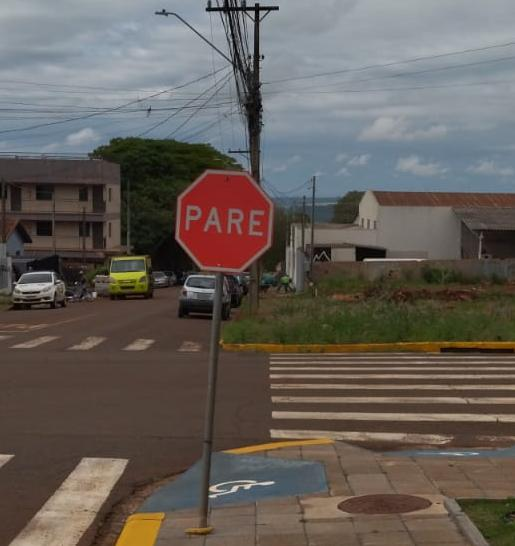
\includegraphics[scale=0.30]{placa.png}
%- endblock

%- block editorial
This is the editorial.
%- endblock
